
% Default to the notebook output style
% Inherit from the specified cell style.
\documentclass[11pt]{article}
    \usepackage[T1]{fontenc}
    % Nicer default font (+ math font) than Computer Modern for most use cases
    \usepackage{mathpazo}

    % Basic figure setup, for now with no caption control since it's done
    % automatically by Pandoc (which extracts ![](path) syntax from Markdown).
    \usepackage{graphicx}
    % We will generate all images so they have a width \maxwidth. This means
    % that they will get their normal width if they fit onto the page, but
    % are scaled down if they would overflow the margins.
    \makeatletter
    \def\maxwidth{\ifdim\Gin@nat@width>\linewidth\linewidth
    \else\Gin@nat@width\fi}
    \makeatother
    \let\Oldincludegraphics\includegraphics
    % Set max figure width to be 80% of text width, for now hardcoded.
    \renewcommand{\includegraphics}[1]{\Oldincludegraphics[width=.8\maxwidth]{#1}}
    % Ensure that by default, figures have no caption (until we provide a
    % proper Figure object with a Caption API and a way to capture that
    % in the conversion process - todo).
    \usepackage{caption}
    \DeclareCaptionLabelFormat{nolabel}{}
    \captionsetup{labelformat=nolabel}

    \usepackage{adjustbox} % Used to constrain images to a maximum size
    \usepackage{xcolor} % Allow colors to be defined
    \usepackage{enumerate} % Needed for markdown enumerations to work
    \usepackage{geometry} % Used to adjust the document margins
    \usepackage{amsmath} % Equations
    \usepackage{amssymb} % Equations
    \usepackage{textcomp} % defines textquotesingle
    % Hack from http://tex.stackexchange.com/a/47451/13684:
    \AtBeginDocument{%
        \def\PYZsq{\textquotesingle}% Upright quotes in Pygmentized code
    }
    \usepackage{upquote} % Upright quotes for verbatim code
    \usepackage{eurosym} % defines \euro
    \usepackage[mathletters]{ucs} % Extended unicode (utf-8) support
    \usepackage[utf8x]{inputenc} % Allow utf-8 characters in the tex document
    \usepackage{fancyvrb} % verbatim replacement that allows latex
    \usepackage{grffile} % extends the file name processing of package graphics
                         % to support a larger range
    % The hyperref package gives us a pdf with properly built
    % internal navigation ('pdf bookmarks' for the table of contents,
    % internal cross-reference links, web links for URLs, etc.)
    \usepackage{hyperref}
    \usepackage{longtable} % longtable support required by pandoc >1.10
    \usepackage{booktabs}  % table support for pandoc > 1.12.2
    \usepackage[inline]{enumitem} % IRkernel/repr support (it uses the enumerate* environment)
    \usepackage[normalem]{ulem} % ulem is needed to support strikethroughs (\sout)
                                % normalem makes italics be italics, not underlines
    \usepackage{mathrsfs}

    % Colors for the hyperref package
    \definecolor{urlcolor}{rgb}{0,.145,.698}
    \definecolor{linkcolor}{rgb}{.71,0.21,0.01}
    \definecolor{citecolor}{rgb}{.12,.54,.11}

    % ANSI colors
    \definecolor{ansi-black}{HTML}{3E424D}
    \definecolor{ansi-black-intense}{HTML}{282C36}
    \definecolor{ansi-red}{HTML}{E75C58}
    \definecolor{ansi-red-intense}{HTML}{B22B31}
    \definecolor{ansi-green}{HTML}{00A250}
    \definecolor{ansi-green-intense}{HTML}{007427}
    \definecolor{ansi-yellow}{HTML}{DDB62B}
    \definecolor{ansi-yellow-intense}{HTML}{B27D12}
    \definecolor{ansi-blue}{HTML}{208FFB}
    \definecolor{ansi-blue-intense}{HTML}{0065CA}
    \definecolor{ansi-magenta}{HTML}{D160C4}
    \definecolor{ansi-magenta-intense}{HTML}{A03196}
    \definecolor{ansi-cyan}{HTML}{60C6C8}
    \definecolor{ansi-cyan-intense}{HTML}{258F8F}
    \definecolor{ansi-white}{HTML}{C5C1B4}
    \definecolor{ansi-white-intense}{HTML}{A1A6B2}
    \definecolor{ansi-default-inverse-fg}{HTML}{FFFFFF}
    \definecolor{ansi-default-inverse-bg}{HTML}{000000}

    % commands and environments needed by pandoc snippets
    % extracted from the output of `pandoc -s`
    \providecommand{\tightlist}{%
      \setlength{\itemsep}{0pt}\setlength{\parskip}{0pt}}
    \DefineVerbatimEnvironment{Highlighting}{Verbatim}{commandchars=\\\{\}}
    % Add ',fontsize=\small' for more characters per line
    \newenvironment{Shaded}{}{}
    \newcommand{\KeywordTok}[1]{\textcolor[rgb]{0.00,0.44,0.13}{\textbf{{#1}}}}
    \newcommand{\DataTypeTok}[1]{\textcolor[rgb]{0.56,0.13,0.00}{{#1}}}
    \newcommand{\DecValTok}[1]{\textcolor[rgb]{0.25,0.63,0.44}{{#1}}}
    \newcommand{\BaseNTok}[1]{\textcolor[rgb]{0.25,0.63,0.44}{{#1}}}
    \newcommand{\FloatTok}[1]{\textcolor[rgb]{0.25,0.63,0.44}{{#1}}}
    \newcommand{\CharTok}[1]{\textcolor[rgb]{0.25,0.44,0.63}{{#1}}}
    \newcommand{\StringTok}[1]{\textcolor[rgb]{0.25,0.44,0.63}{{#1}}}
    \newcommand{\CommentTok}[1]{\textcolor[rgb]{0.38,0.63,0.69}{\textit{{#1}}}}
    \newcommand{\OtherTok}[1]{\textcolor[rgb]{0.00,0.44,0.13}{{#1}}}
    \newcommand{\AlertTok}[1]{\textcolor[rgb]{1.00,0.00,0.00}{\textbf{{#1}}}}
    \newcommand{\FunctionTok}[1]{\textcolor[rgb]{0.02,0.16,0.49}{{#1}}}
    \newcommand{\RegionMarkerTok}[1]{{#1}}
    \newcommand{\ErrorTok}[1]{\textcolor[rgb]{1.00,0.00,0.00}{\textbf{{#1}}}}
    \newcommand{\NormalTok}[1]{{#1}}

    % Additional commands for more recent versions of Pandoc
    \newcommand{\ConstantTok}[1]{\textcolor[rgb]{0.53,0.00,0.00}{{#1}}}
    \newcommand{\SpecialCharTok}[1]{\textcolor[rgb]{0.25,0.44,0.63}{{#1}}}
    \newcommand{\VerbatimStringTok}[1]{\textcolor[rgb]{0.25,0.44,0.63}{{#1}}}
    \newcommand{\SpecialStringTok}[1]{\textcolor[rgb]{0.73,0.40,0.53}{{#1}}}
    \newcommand{\ImportTok}[1]{{#1}}
    \newcommand{\DocumentationTok}[1]{\textcolor[rgb]{0.73,0.13,0.13}{\textit{{#1}}}}
    \newcommand{\AnnotationTok}[1]{\textcolor[rgb]{0.38,0.63,0.69}{\textbf{\textit{{#1}}}}}
    \newcommand{\CommentVarTok}[1]{\textcolor[rgb]{0.38,0.63,0.69}{\textbf{\textit{{#1}}}}}
    \newcommand{\VariableTok}[1]{\textcolor[rgb]{0.10,0.09,0.49}{{#1}}}
    \newcommand{\ControlFlowTok}[1]{\textcolor[rgb]{0.00,0.44,0.13}{\textbf{{#1}}}}
    \newcommand{\OperatorTok}[1]{\textcolor[rgb]{0.40,0.40,0.40}{{#1}}}
    \newcommand{\BuiltInTok}[1]{{#1}}
    \newcommand{\ExtensionTok}[1]{{#1}}
    \newcommand{\PreprocessorTok}[1]{\textcolor[rgb]{0.74,0.48,0.00}{{#1}}}
    \newcommand{\AttributeTok}[1]{\textcolor[rgb]{0.49,0.56,0.16}{{#1}}}
    \newcommand{\InformationTok}[1]{\textcolor[rgb]{0.38,0.63,0.69}{\textbf{\textit{{#1}}}}}
    \newcommand{\WarningTok}[1]{\textcolor[rgb]{0.38,0.63,0.69}{\textbf{\textit{{#1}}}}}


    % Define a nice break command that doesn't care if a line doesn't already
    % exist.
    \def\br{\hspace*{\fill} \\* }
    % Math Jax compatibility definitions
    \def\gt{>}
    \def\lt{<}
    \let\Oldtex\TeX
    \let\Oldlatex\LaTeX
    \renewcommand{\TeX}{\textrm{\Oldtex}}
    \renewcommand{\LaTeX}{\textrm{\Oldlatex}}
    % Document parameters
    % Document title
    \title{Monitoring the Saharan Air Layer using Satellite Applications}
    \author{Rebekah Esmaili, \href{mailto:rebekah@stcnet.com}{rebekah@stcnet.com}
    \\ Science and Technology Corportation}

    %\href{https://mybinder.org/v2/gh/resmaili/nucaps-sal/master} {Click to Launch Code} }

    \date{29 September 2019}

    % Pygments definitions

\makeatletter
\def\PY@reset{\let\PY@it=\relax \let\PY@bf=\relax%
    \let\PY@ul=\relax \let\PY@tc=\relax%
    \let\PY@bc=\relax \let\PY@ff=\relax}
\def\PY@tok#1{\csname PY@tok@#1\endcsname}
\def\PY@toks#1+{\ifx\relax#1\empty\else%
    \PY@tok{#1}\expandafter\PY@toks\fi}
\def\PY@do#1{\PY@bc{\PY@tc{\PY@ul{%
    \PY@it{\PY@bf{\PY@ff{#1}}}}}}}
\def\PY#1#2{\PY@reset\PY@toks#1+\relax+\PY@do{#2}}

\expandafter\def\csname PY@tok@w\endcsname{\def\PY@tc##1{\textcolor[rgb]{0.73,0.73,0.73}{##1}}}
\expandafter\def\csname PY@tok@c\endcsname{\let\PY@it=\textit\def\PY@tc##1{\textcolor[rgb]{0.25,0.50,0.50}{##1}}}
\expandafter\def\csname PY@tok@cp\endcsname{\def\PY@tc##1{\textcolor[rgb]{0.74,0.48,0.00}{##1}}}
\expandafter\def\csname PY@tok@k\endcsname{\let\PY@bf=\textbf\def\PY@tc##1{\textcolor[rgb]{0.00,0.50,0.00}{##1}}}
\expandafter\def\csname PY@tok@kp\endcsname{\def\PY@tc##1{\textcolor[rgb]{0.00,0.50,0.00}{##1}}}
\expandafter\def\csname PY@tok@kt\endcsname{\def\PY@tc##1{\textcolor[rgb]{0.69,0.00,0.25}{##1}}}
\expandafter\def\csname PY@tok@o\endcsname{\def\PY@tc##1{\textcolor[rgb]{0.40,0.40,0.40}{##1}}}
\expandafter\def\csname PY@tok@ow\endcsname{\let\PY@bf=\textbf\def\PY@tc##1{\textcolor[rgb]{0.67,0.13,1.00}{##1}}}
\expandafter\def\csname PY@tok@nb\endcsname{\def\PY@tc##1{\textcolor[rgb]{0.00,0.50,0.00}{##1}}}
\expandafter\def\csname PY@tok@nf\endcsname{\def\PY@tc##1{\textcolor[rgb]{0.00,0.00,1.00}{##1}}}
\expandafter\def\csname PY@tok@nc\endcsname{\let\PY@bf=\textbf\def\PY@tc##1{\textcolor[rgb]{0.00,0.00,1.00}{##1}}}
\expandafter\def\csname PY@tok@nn\endcsname{\let\PY@bf=\textbf\def\PY@tc##1{\textcolor[rgb]{0.00,0.00,1.00}{##1}}}
\expandafter\def\csname PY@tok@ne\endcsname{\let\PY@bf=\textbf\def\PY@tc##1{\textcolor[rgb]{0.82,0.25,0.23}{##1}}}
\expandafter\def\csname PY@tok@nv\endcsname{\def\PY@tc##1{\textcolor[rgb]{0.10,0.09,0.49}{##1}}}
\expandafter\def\csname PY@tok@no\endcsname{\def\PY@tc##1{\textcolor[rgb]{0.53,0.00,0.00}{##1}}}
\expandafter\def\csname PY@tok@nl\endcsname{\def\PY@tc##1{\textcolor[rgb]{0.63,0.63,0.00}{##1}}}
\expandafter\def\csname PY@tok@ni\endcsname{\let\PY@bf=\textbf\def\PY@tc##1{\textcolor[rgb]{0.60,0.60,0.60}{##1}}}
\expandafter\def\csname PY@tok@na\endcsname{\def\PY@tc##1{\textcolor[rgb]{0.49,0.56,0.16}{##1}}}
\expandafter\def\csname PY@tok@nt\endcsname{\let\PY@bf=\textbf\def\PY@tc##1{\textcolor[rgb]{0.00,0.50,0.00}{##1}}}
\expandafter\def\csname PY@tok@nd\endcsname{\def\PY@tc##1{\textcolor[rgb]{0.67,0.13,1.00}{##1}}}
\expandafter\def\csname PY@tok@s\endcsname{\def\PY@tc##1{\textcolor[rgb]{0.73,0.13,0.13}{##1}}}
\expandafter\def\csname PY@tok@sd\endcsname{\let\PY@it=\textit\def\PY@tc##1{\textcolor[rgb]{0.73,0.13,0.13}{##1}}}
\expandafter\def\csname PY@tok@si\endcsname{\let\PY@bf=\textbf\def\PY@tc##1{\textcolor[rgb]{0.73,0.40,0.53}{##1}}}
\expandafter\def\csname PY@tok@se\endcsname{\let\PY@bf=\textbf\def\PY@tc##1{\textcolor[rgb]{0.73,0.40,0.13}{##1}}}
\expandafter\def\csname PY@tok@sr\endcsname{\def\PY@tc##1{\textcolor[rgb]{0.73,0.40,0.53}{##1}}}
\expandafter\def\csname PY@tok@ss\endcsname{\def\PY@tc##1{\textcolor[rgb]{0.10,0.09,0.49}{##1}}}
\expandafter\def\csname PY@tok@sx\endcsname{\def\PY@tc##1{\textcolor[rgb]{0.00,0.50,0.00}{##1}}}
\expandafter\def\csname PY@tok@m\endcsname{\def\PY@tc##1{\textcolor[rgb]{0.40,0.40,0.40}{##1}}}
\expandafter\def\csname PY@tok@gh\endcsname{\let\PY@bf=\textbf\def\PY@tc##1{\textcolor[rgb]{0.00,0.00,0.50}{##1}}}
\expandafter\def\csname PY@tok@gu\endcsname{\let\PY@bf=\textbf\def\PY@tc##1{\textcolor[rgb]{0.50,0.00,0.50}{##1}}}
\expandafter\def\csname PY@tok@gd\endcsname{\def\PY@tc##1{\textcolor[rgb]{0.63,0.00,0.00}{##1}}}
\expandafter\def\csname PY@tok@gi\endcsname{\def\PY@tc##1{\textcolor[rgb]{0.00,0.63,0.00}{##1}}}
\expandafter\def\csname PY@tok@gr\endcsname{\def\PY@tc##1{\textcolor[rgb]{1.00,0.00,0.00}{##1}}}
\expandafter\def\csname PY@tok@ge\endcsname{\let\PY@it=\textit}
\expandafter\def\csname PY@tok@gs\endcsname{\let\PY@bf=\textbf}
\expandafter\def\csname PY@tok@gp\endcsname{\let\PY@bf=\textbf\def\PY@tc##1{\textcolor[rgb]{0.00,0.00,0.50}{##1}}}
\expandafter\def\csname PY@tok@go\endcsname{\def\PY@tc##1{\textcolor[rgb]{0.53,0.53,0.53}{##1}}}
\expandafter\def\csname PY@tok@gt\endcsname{\def\PY@tc##1{\textcolor[rgb]{0.00,0.27,0.87}{##1}}}
\expandafter\def\csname PY@tok@err\endcsname{\def\PY@bc##1{\setlength{\fboxsep}{0pt}\fcolorbox[rgb]{1.00,0.00,0.00}{1,1,1}{\strut ##1}}}
\expandafter\def\csname PY@tok@kc\endcsname{\let\PY@bf=\textbf\def\PY@tc##1{\textcolor[rgb]{0.00,0.50,0.00}{##1}}}
\expandafter\def\csname PY@tok@kd\endcsname{\let\PY@bf=\textbf\def\PY@tc##1{\textcolor[rgb]{0.00,0.50,0.00}{##1}}}
\expandafter\def\csname PY@tok@kn\endcsname{\let\PY@bf=\textbf\def\PY@tc##1{\textcolor[rgb]{0.00,0.50,0.00}{##1}}}
\expandafter\def\csname PY@tok@kr\endcsname{\let\PY@bf=\textbf\def\PY@tc##1{\textcolor[rgb]{0.00,0.50,0.00}{##1}}}
\expandafter\def\csname PY@tok@bp\endcsname{\def\PY@tc##1{\textcolor[rgb]{0.00,0.50,0.00}{##1}}}
\expandafter\def\csname PY@tok@fm\endcsname{\def\PY@tc##1{\textcolor[rgb]{0.00,0.00,1.00}{##1}}}
\expandafter\def\csname PY@tok@vc\endcsname{\def\PY@tc##1{\textcolor[rgb]{0.10,0.09,0.49}{##1}}}
\expandafter\def\csname PY@tok@vg\endcsname{\def\PY@tc##1{\textcolor[rgb]{0.10,0.09,0.49}{##1}}}
\expandafter\def\csname PY@tok@vi\endcsname{\def\PY@tc##1{\textcolor[rgb]{0.10,0.09,0.49}{##1}}}
\expandafter\def\csname PY@tok@vm\endcsname{\def\PY@tc##1{\textcolor[rgb]{0.10,0.09,0.49}{##1}}}
\expandafter\def\csname PY@tok@sa\endcsname{\def\PY@tc##1{\textcolor[rgb]{0.73,0.13,0.13}{##1}}}
\expandafter\def\csname PY@tok@sb\endcsname{\def\PY@tc##1{\textcolor[rgb]{0.73,0.13,0.13}{##1}}}
\expandafter\def\csname PY@tok@sc\endcsname{\def\PY@tc##1{\textcolor[rgb]{0.73,0.13,0.13}{##1}}}
\expandafter\def\csname PY@tok@dl\endcsname{\def\PY@tc##1{\textcolor[rgb]{0.73,0.13,0.13}{##1}}}
\expandafter\def\csname PY@tok@s2\endcsname{\def\PY@tc##1{\textcolor[rgb]{0.73,0.13,0.13}{##1}}}
\expandafter\def\csname PY@tok@sh\endcsname{\def\PY@tc##1{\textcolor[rgb]{0.73,0.13,0.13}{##1}}}
\expandafter\def\csname PY@tok@s1\endcsname{\def\PY@tc##1{\textcolor[rgb]{0.73,0.13,0.13}{##1}}}
\expandafter\def\csname PY@tok@mb\endcsname{\def\PY@tc##1{\textcolor[rgb]{0.40,0.40,0.40}{##1}}}
\expandafter\def\csname PY@tok@mf\endcsname{\def\PY@tc##1{\textcolor[rgb]{0.40,0.40,0.40}{##1}}}
\expandafter\def\csname PY@tok@mh\endcsname{\def\PY@tc##1{\textcolor[rgb]{0.40,0.40,0.40}{##1}}}
\expandafter\def\csname PY@tok@mi\endcsname{\def\PY@tc##1{\textcolor[rgb]{0.40,0.40,0.40}{##1}}}
\expandafter\def\csname PY@tok@il\endcsname{\def\PY@tc##1{\textcolor[rgb]{0.40,0.40,0.40}{##1}}}
\expandafter\def\csname PY@tok@mo\endcsname{\def\PY@tc##1{\textcolor[rgb]{0.40,0.40,0.40}{##1}}}
\expandafter\def\csname PY@tok@ch\endcsname{\let\PY@it=\textit\def\PY@tc##1{\textcolor[rgb]{0.25,0.50,0.50}{##1}}}
\expandafter\def\csname PY@tok@cm\endcsname{\let\PY@it=\textit\def\PY@tc##1{\textcolor[rgb]{0.25,0.50,0.50}{##1}}}
\expandafter\def\csname PY@tok@cpf\endcsname{\let\PY@it=\textit\def\PY@tc##1{\textcolor[rgb]{0.25,0.50,0.50}{##1}}}
\expandafter\def\csname PY@tok@c1\endcsname{\let\PY@it=\textit\def\PY@tc##1{\textcolor[rgb]{0.25,0.50,0.50}{##1}}}
\expandafter\def\csname PY@tok@cs\endcsname{\let\PY@it=\textit\def\PY@tc##1{\textcolor[rgb]{0.25,0.50,0.50}{##1}}}

\def\PYZbs{\char`\\}
\def\PYZus{\char`\_}
\def\PYZob{\char`\{}
\def\PYZcb{\char`\}}
\def\PYZca{\char`\^}
\def\PYZam{\char`\&}
\def\PYZlt{\char`\<}
\def\PYZgt{\char`\>}
\def\PYZsh{\char`\#}
\def\PYZpc{\char`\%}
\def\PYZdl{\char`\$}
\def\PYZhy{\char`\-}
\def\PYZsq{\char`\'}
\def\PYZdq{\char`\"}
\def\PYZti{\char`\~}
% for compatibility with earlier versions
\def\PYZat{@}
\def\PYZlb{[}
\def\PYZrb{]}
\makeatother

    % Exact colors from NB
    \definecolor{incolor}{rgb}{0.0, 0.0, 0.5}
    \definecolor{outcolor}{rgb}{0.545, 0.0, 0.0}

    % Prevent overflowing lines due to hard-to-break entities
    \sloppy
    % Setup hyperref package
    \hypersetup{
      breaklinks=true,  % so long urls are correctly broken across lines
      colorlinks=true,
      urlcolor=urlcolor,
      linkcolor=linkcolor,
      citecolor=citecolor,
      }
    % Slightly bigger margins than the latex defaults

    \geometry{verbose,tmargin=1in,bmargin=1in,lmargin=.75in,rmargin=.75in}


    \begin{document}
    \maketitle


\begin{figure}[h!]
\centering
\href{https://mybinder.org/v2/gh/resmaili/nucaps-sal/master}{
\includegraphics{images/badge_logo.jpg}}
\caption*{\href{https://mybinder.org/v2/gh/resmaili/nucaps-sal/master}{This tutorial is interactive, click to launch code!}}
\end{figure}


\begin{figure}
\centering
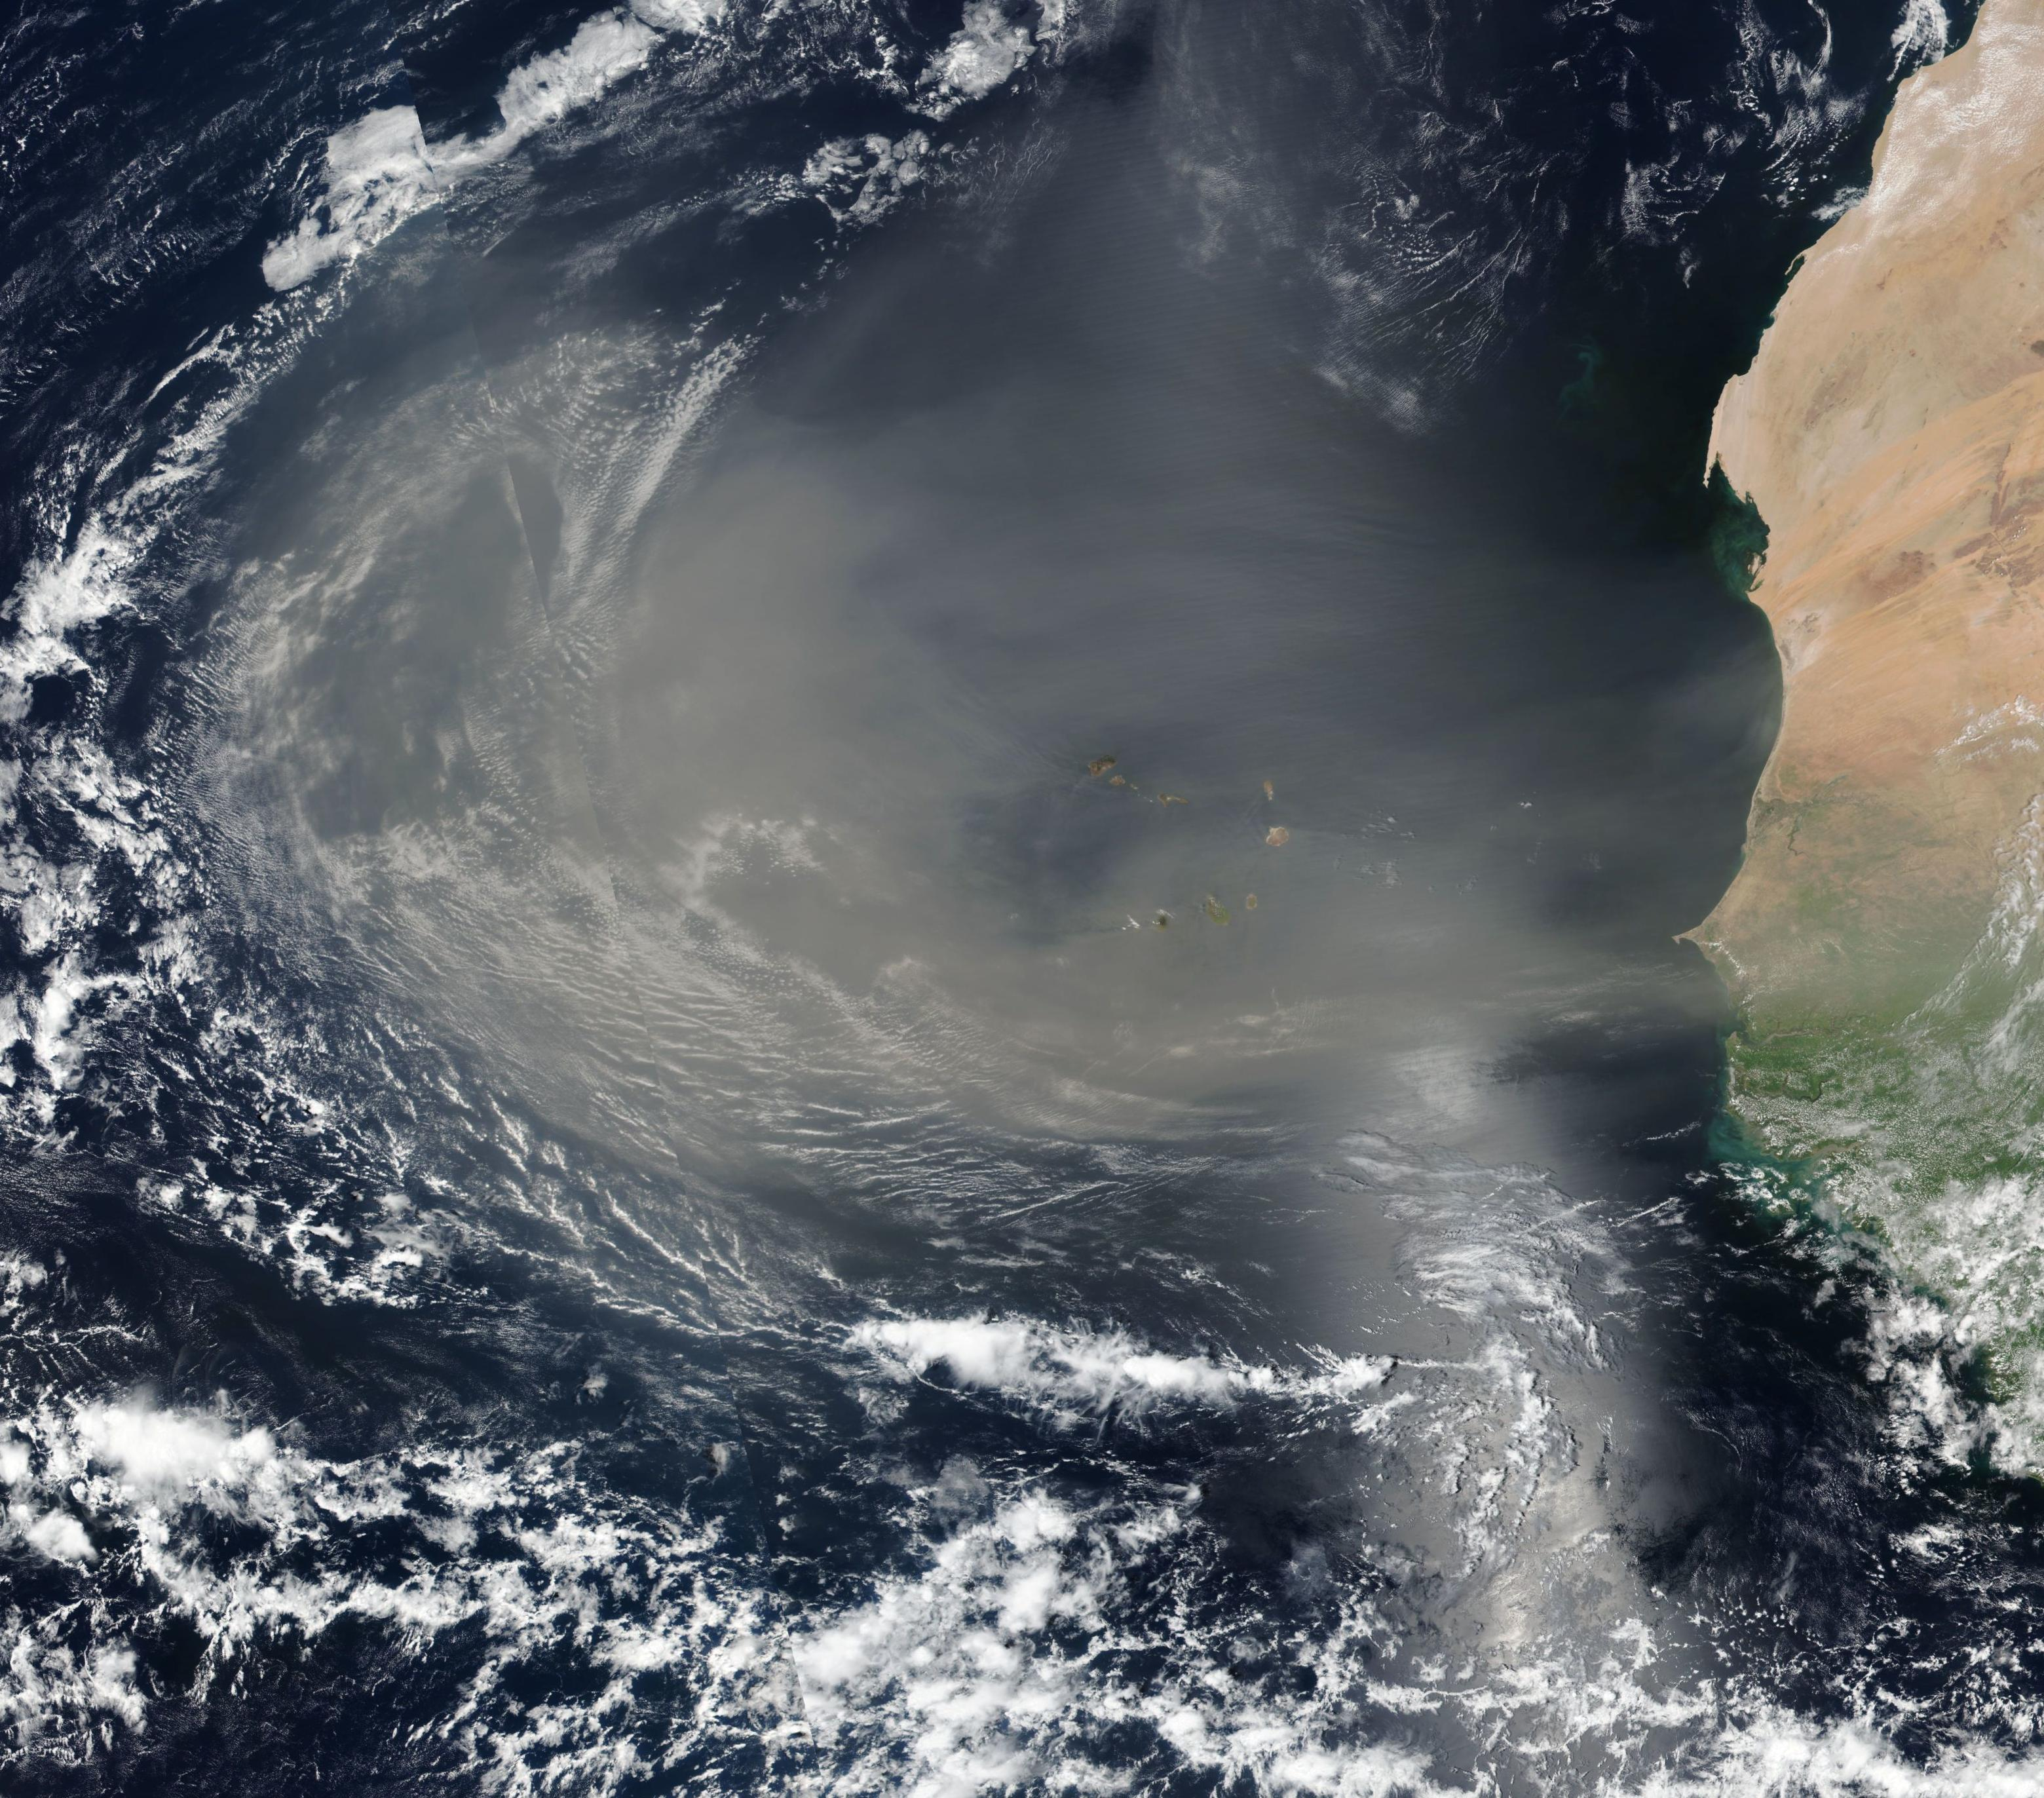
\includegraphics{images/SAL.jpeg}
\caption{Figure \ref{fig:sal}: A SAL outflow on September 15, 2019}
\label{fig:sal}
\end{figure}

\section{What is the Saharan Air
Layer?}\label{what-is-the-saharan-air-layer}

The Saharan Air Layer (SAL) is a warm and dry pocket of air that
originates over the Saharan Desert and propagates over the Atlantic. The
SAL extends from 850-500mb and has very steep lapse rates, thus capping
the moist, tropical marine air below. This can potentially suppress tropical
cyclone formation. The SAL is a potential hazard because it can
transport dust to populated regions across the Atlantic, reducing
air quality over the Caribbean and eastern United States. This can increase allergies and asthma in sensitive populations.

Figure \ref{fig:sal} shows a SAL outflow on September 15, 2018 using the VIIRS
instrument from the Suomi NPP satellite. This SAL event reached the
Caribbean on September 20, 2018. The SAL can be detected from space by examining visible and infrared imagery from a variety of sensors on satellite platform, such as the ABI (GOES-16), SEVIRI (Meteosat-9/-10), VIIRS (Suomi NPP, NOAA-20), and AVHRR (MetOp-A, -B, -C). The horizontal extent of the SAL can be monitored using dust RGB imagery, channel differencing (e.g., 10.33 µm -- 12.30 µm), and Aerosol Optical Depth (AOD) retrievals. Additionally, microwave and infrared sounding (CrIS, ATMS, AMSU, and IASI) are particularly useful for SAL monitoring because sounder products can detect both the horizontal and vertical distribution of the dry air mass.

\section{What is NUCAPS?}\label{what-is-nucaps}

The NOAA Unique Combined Atmospheric Processing System (NUCAPS)
operationally produces atmospheric sounding products from the Suomi
National-Polar-orbiting Partnership (Suomi NPP) and NOAA-20 polar orbiting
satellites. From each satellite, NUCAPS provides global, twice-daily
scans and is available in near real-time. NUCAPS provides vertical profiles
of temperature, humidity, and trace gases such as ozone, methane, and
carbon monoxide.

NUCAPS humidity profiles is useful for studying the vertical profile of
SAL and to verify model predictions for SAL propagation.

\section{Where can I get NUCAPS
datasets?}\label{where-can-i-get-nucaps-datasets}

For researchers, NOAA-20 and Suomi NPP NUCAPS data can be ordered from
\href{https://www.bou.class.noaa.gov/saa/products/search?sub_id=0\&datatype_family=JPSS_SND\&submit.x=24\&submit.y=7}{NOAA
CLASS}, under the JPSS Sound Products (JPSS\_SND) drop down menu. For operational forecasters, NOAA-20 NUCAPS is available within 20 mintes through in AWIPS.

\section{How can I visualize NUCAPS
datasets?}\label{how-can-i-visualize-nucaps-datasets}

The daily ascending and descending overpasses can be viewed online via
the
\href{https://www.star.nesdis.noaa.gov/jpss/EDRs/products_Soundings_N20.php}{NOAA/STAR}. Additionally, skew-T visualizations are routinely produced by \href{https://www.ospo.noaa.gov/Products/atmosphere/soundings/nucaps/pskewt/USACON.html}{NOAA/OSPO} for NOAA-20, Suomi NPP, and MetOp series.

Below is a short tutorial on how to display NUCAPS using Python and
Jupyter Notebooks. This tutorial is intended to be a beginner-friendly exercise. So, even if
you are not a Python programmer, you may be able to port it to another
language of choice.

\subsection{Objectives}\label{objectives}

\begin{itemize}
\tightlist
\item
  Open and inspect a single NUCAPS file, containing one swath of data
\item
  Create maps and vertical cross section plots
\item
  Combine many single files onto a map
\end{itemize}

First, we will import several 'helper' libraries to process the data.
the '\#' symbole indicates comments and will not run with the code.

    \begin{Verbatim}[commandchars=\\\{\}]
{\color{incolor}In [{\color{incolor}109}]:} \PY{k+kn}{import} \PY{n+nn}{numpy} \PY{k}{as} \PY{n+nn}{np}                         \PY{c+c1}{\PYZsh{} To perform array operations}
          \PY{k+kn}{import} \PY{n+nn}{cartopy}\PY{n+nn}{.}\PY{n+nn}{crs} \PY{k}{as} \PY{n+nn}{ccrs}                 \PY{c+c1}{\PYZsh{} To create map projections for plots}
          \PY{k+kn}{import} \PY{n+nn}{cartopy}\PY{n+nn}{.}\PY{n+nn}{feature} \PY{k}{as} \PY{n+nn}{cfeature}         \PY{c+c1}{\PYZsh{} To add maps to plots}
          \PY{k+kn}{from} \PY{n+nn}{glob} \PY{k}{import} \PY{n}{glob}                      \PY{c+c1}{\PYZsh{} Search all files in a directory}
          \PY{k+kn}{import} \PY{n+nn}{matplotlib}\PY{n+nn}{.}\PY{n+nn}{pyplot} \PY{k}{as} \PY{n+nn}{plt}            \PY{c+c1}{\PYZsh{} Main plotting library}
          \PY{k+kn}{import} \PY{n+nn}{xarray} \PY{k}{as} \PY{n+nn}{xr}                        \PY{c+c1}{\PYZsh{} For working with netCDF files}

          \PY{n}{plt}\PY{o}{.}\PY{n}{rcParams}\PY{p}{[}\PY{l+s+s1}{\PYZsq{}}\PY{l+s+s1}{figure.figsize}\PY{l+s+s1}{\PYZsq{}}\PY{p}{]} \PY{o}{=} \PY{p}{[}\PY{l+m+mi}{15}\PY{p}{,} \PY{l+m+mi}{10}\PY{p}{]} \PY{c+c1}{\PYZsh{} Sets all figures in document to be 15\PYZdq{}x10\PYZdq{}}
          \PY{n}{plt}\PY{o}{.}\PY{n}{rcParams}\PY{o}{.}\PY{n}{update}\PY{p}{(}\PY{p}{\PYZob{}}\PY{l+s+s1}{\PYZsq{}}\PY{l+s+s1}{font.size}\PY{l+s+s1}{\PYZsq{}}\PY{p}{:} \PY{l+m+mi}{21}\PY{p}{\PYZcb{}}\PY{p}{)}     \PY{c+c1}{\PYZsh{} Sets fontsize in document to 21pts}
\end{Verbatim}

    \subsection{The JPSS file naming
scheme}\label{the-jpss-file-naming-scheme}

The code below will read in a single netCDF file. The file names are
very long!

\textbf{NUCAPS-EDR\_v2r0\_npp\_s201809201634390\_e201809201635090\_c201809201739220.nc}

But there's a general trend in the filenames, so using the underscore
(\_) as a seperator:

\begin{itemize}
\tightlist
\item
  NUCAPS-EDR: product
\item
  v2r0: algorithm
\item
  npp: satellite
\item
  s201809201634390: start time
\item
  e201809201635090: end time
\item
  c201809201739220: creation time
\end{itemize}

By looking at the start and end times of the name, we see that
the file contains 1 minute of NUCAPS data collected from the Suomi NPP
sensors.

\subsection{Importing a single granule of data using
xarray}\label{importing-a-single-granule-of-data-using-xarray}

Using the open\_dataset command in xarray, let's import the file. Note
that we need the decode\_times option to be false, because xarray
expects them to be stored in miliseconds and the NUCAPS files stores
them in nanoseconds.

    \begin{Verbatim}[commandchars=\\\{\}]
      {\color{incolor}In [{\color{incolor}49}]:} \PY{c+c1}{\PYZsh{} Read in a single NUCAPS netcdf file }
               \PY{c+c1}{\PYZsh{} Set decode time = false (the time doesnt follow standard formatting)}
         \PY{n}{fname} \PY{o}{=} \PY{l+s+s1}{\PYZsq{}}\PY{l+s+s1}{sal/NUCAPS\PYZhy{}EDR\PYZus{}v2r0\PYZus{}npp\PYZus{}s201809201638230\PYZus{}e201809201638530\PYZus{}c201809201742190.nc}\PY{l+s+s1}{\PYZsq{}}
         \PY{n}{nucaps} \PY{o}{=} \PY{n}{xr}\PY{o}{.}\PY{n}{open\PYZus{}dataset}\PY{p}{(}\PY{n}{fname}\PY{p}{,} \PY{n}{decode\PYZus{}times}\PY{o}{=}\PY{k+kc}{False}\PY{p}{)}
\end{Verbatim}

    \begin{Verbatim}[commandchars=\\\{\}]
{\color{incolor}In [{\color{incolor}82}]:} \PY{c+c1}{\PYZsh{} Uncomment to inspect the file contents...}
         \PY{n}{nucaps}
\end{Verbatim}

\begin{Verbatim}[commandchars=\\\{\}]
{\color{outcolor}Out[{\color{outcolor}82}]:} <xarray.Dataset>
         Dimensions:               (Number\_of\_Cloud\_Emis\_Hing\_Pts: 100, Number\_of\_Cloud\_Layers: 8,
            Number\_of\_CrIS\_FORs: 120, Number\_of\_Ispares: 129, Number\_of\_MW\_Spectral\_Pts: 16,
            Number\_of\_P\_Levels: 100, Number\_of\_Rspares: 262, Number\_of\_Stability\_Parameters: 16,
            Number\_of\_Surf\_Emis\_Hinge\_Pts: 100)
         Coordinates:
             Time                  (Number\_of\_CrIS\_FORs) float64 {\ldots}
             Latitude              (Number\_of\_CrIS\_FORs) float32 {\ldots}
             Longitude             (Number\_of\_CrIS\_FORs) float32 {\ldots}
             Pressure              (Number\_of\_CrIS\_FORs, Number\_of\_P\_Levels) float32 {\ldots}
             Effective\_Pressure    (Number\_of\_CrIS\_FORs, Number\_of\_P\_Levels) float32 {\ldots}
         Dimensions without coordinates: Number\_of\_Cloud\_Emis\_Hing\_Pts, Number\_of\_Cloud\_Layers,
          Number\_of\_CrIS\_FORs, Number\_of\_Ispares, Number\_of\_MW\_Spectral\_Pts,
          Number\_of\_P\_Levels, Number\_of\_Rspares, Number\_of\_Stability\_Parameters,
          Number\_of\_Surf\_Emis\_Hinge\_Pts
         Data variables:
             quality\_information   |S1 {\ldots}
             CrIS\_FORs             (Number\_of\_CrIS\_FORs) float64 {\ldots}
             View\_Angle            (Number\_of\_CrIS\_FORs) float32 {\ldots}
             Satellite\_Height      (Number\_of\_CrIS\_FORs) float32 {\ldots}
             FG\_Mean\_CO2           (Number\_of\_CrIS\_FORs) float32 {\ldots}
             Mean\_CO2              (Number\_of\_CrIS\_FORs) float32 {\ldots}
             Solar\_Zenith          (Number\_of\_CrIS\_FORs) float32 {\ldots}
             Ascending\_Descending  (Number\_of\_CrIS\_FORs) float32 {\ldots}
             Topography            (Number\_of\_CrIS\_FORs) float32 {\ldots}
             Land\_Fraction         (Number\_of\_CrIS\_FORs) float32 {\ldots}
             Surface\_Pressure      (Number\_of\_CrIS\_FORs) float32 {\ldots}
             Skin\_Temperature      (Number\_of\_CrIS\_FORs) float32 {\ldots}
             MIT\_Skin\_Temperature  (Number\_of\_CrIS\_FORs) float32 {\ldots}
             FG\_Skin\_Temperature   (Number\_of\_CrIS\_FORs) float32 {\ldots}
             MW\_Surface\_Class      (Number\_of\_CrIS\_FORs) float32 {\ldots}
             ...
             Ispare\_Field          (Number\_of\_CrIS\_FORs, Number\_of\_Ispares) float64 {\ldots}
             Rspare\_Field          (Number\_of\_CrIS\_FORs, Number\_of\_Rspares) float32 {\ldots}
             Cloud\_Top\_Pressure    (Number\_of\_CrIS\_FORs, Number\_of\_Cloud\_Layers) float32 {\ldots}
             Cloud\_Top\_Fraction    (Number\_of\_CrIS\_FORs, Number\_of\_Cloud\_Layers) float32 {\ldots}
             Temperature           (Number\_of\_CrIS\_FORs, Number\_of\_P\_Levels) float32 {\ldots}
             MIT\_Temperature       (Number\_of\_CrIS\_FORs, Number\_of\_P\_Levels) float32 {\ldots}
             FG\_Temperature        (Number\_of\_CrIS\_FORs, Number\_of\_P\_Levels) float32 {\ldots}
             H2O                   (Number\_of\_CrIS\_FORs, Number\_of\_P\_Levels) float32 {\ldots}
             ...
\end{Verbatim}

    \subsection{Creating a simple map}\label{creating-a-simple-map}

If successfully imported, the command above will display the dimensions,
coordinates, and available variables to plot. First, we will make a map
showing where this granule is by plotting the latitude and logitude
coordinates. NUCAPS data is saved as a 120 field of regards (FORs). This
is stored as the "CrIS\_FORs" coordinate in the NUCAPS netCDF file. Each
FOR is 50km at nadir and 150km at the scan edge.

    \begin{Verbatim}[commandchars=\\\{\}]
{\color{incolor}In [{\color{incolor}114}]:} \PY{c+c1}{\PYZsh{} Initiate the plot}
          \PY{n}{fig} \PY{o}{=} \PY{n}{plt}\PY{o}{.}\PY{n}{figure}\PY{p}{(}\PY{n}{figsize}\PY{o}{=}\PY{p}{(}\PY{l+m+mi}{15}\PY{p}{,} \PY{l+m+mi}{10}\PY{p}{)}\PY{p}{)}

          \PY{c+c1}{\PYZsh{} Adds a map to the plot}
          \PY{n}{ax}\PY{o}{=}\PY{n}{plt}\PY{o}{.}\PY{n}{axes}\PY{p}{(}\PY{n}{projection}\PY{o}{=}\PY{n}{ccrs}\PY{o}{.}\PY{n}{PlateCarree}\PY{p}{(}\PY{p}{)}\PY{p}{)}
          \PY{n}{ax}\PY{o}{.}\PY{n}{coastlines}\PY{p}{(}\PY{l+s+s1}{\PYZsq{}}\PY{l+s+s1}{50m}\PY{l+s+s1}{\PYZsq{}}\PY{p}{)}

          \PY{c+c1}{\PYZsh{} Plots the latitude and longitude of the NUCAPS data}
          \PY{n}{plt}\PY{o}{.}\PY{n}{scatter}\PY{p}{(}\PY{n}{nucaps}\PY{p}{[}\PY{l+s+s1}{\PYZsq{}}\PY{l+s+s1}{Longitude}\PY{l+s+s1}{\PYZsq{}}\PY{p}{]}\PY{p}{,} \PY{n}{nucaps}\PY{p}{[}\PY{l+s+s1}{\PYZsq{}}\PY{l+s+s1}{Latitude}\PY{l+s+s1}{\PYZsq{}}\PY{p}{]}\PY{p}{,} \PY{n}{c}\PY{o}{=}\PY{n}{nucaps}\PY{p}{[}\PY{l+s+s1}{\PYZsq{}}\PY{l+s+s1}{CrIS\PYZus{}FORs}\PY{l+s+s1}{\PYZsq{}}\PY{p}{]}\PY{p}{)}

          \PY{n}{plt}\PY{o}{.}\PY{n}{colorbar}\PY{p}{(}\PY{n}{orientation}\PY{o}{=}\PY{l+s+s1}{\PYZsq{}}\PY{l+s+s1}{horizontal}\PY{l+s+s1}{\PYZsq{}}\PY{p}{)}

          \PY{c+c1}{\PYZsh{} Expands axes}
          \PY{n}{ax}\PY{o}{.}\PY{n}{set\PYZus{}ylim}\PY{p}{(}\PY{o}{\PYZhy{}}\PY{l+m+mi}{5}\PY{p}{,} \PY{l+m+mi}{25}\PY{p}{)}
          \PY{n}{ax}\PY{o}{.}\PY{n}{set\PYZus{}xlim}\PY{p}{(}\PY{o}{\PYZhy{}}\PY{l+m+mi}{90}\PY{p}{,} \PY{l+m+mi}{0}\PY{p}{)}

          \PY{c+c1}{\PYZsh{} Display plot}
          \PY{n}{plt}\PY{o}{.}\PY{n}{show}\PY{p}{(}\PY{p}{)}
\end{Verbatim}

    \begin{center}
    \adjustimage{max size={0.9\linewidth}{0.9\paperheight}}{JSC_SAL_tutorial_files/JSC_SAL_tutorial_6_0.png}
    \end{center}
    { \hspace*{\fill} \\}

    From above, the 120 FORs are numbered linearly, starting at one in the
lower left of the swath, increase to the right, resetting to a new row
with every 30th observation.

\subsection{Plotting a vertical profile of water vapor to examine
the SAL
structure}\label{plotting-a-vertical-profiles-of-water-vapor-to-examine-the-sal-structure}

From the list of data variables, we have access to vertical profiles of temperature, H$_{2}$O, O$_{3}$, CO, etc. Since the SAL is dry, we will see a dry layer when looking at the vertical profiles for each FOR.

To make this plot, we have to make sure all the variables are the same dimensions. By printing below, we'll see that the CRIS\_FORs are one-dimensional while pressure and H$_{2}$O are two-dimensional:

\begin{Verbatim}[commandchars=\\\{\}]
{\color{incolor}In [{\color{incolor}52}]:} \PY{n+nb}{print}\PY{p}{(}\PY{n}{nucaps}\PY{p}{[}\PY{l+s+s1}{\PYZsq{}}\PY{l+s+s1}{Pressure}\PY{l+s+s1}{\PYZsq{}}\PY{p}{]}\PY{o}{.}\PY{n}{shape}\PY{p}{,} \PY{n}{nucaps}\PY{p}{[}\PY{l+s+s1}{\PYZsq{}}\PY{l+s+s1}{H2O}\PY{l+s+s1}{\PYZsq{}}\PY{p}{]}\PY{o}{.}\PY{n}{shape}\PY{p}{,} \PY{n}{nucaps}\PY{p}{[}\PY{l+s+s1}{\PYZsq{}}\PY{l+s+s1}{CrIS\PYZus{}FORs}\PY{l+s+s1}{\PYZsq{}}\PY{p}{]}\PY{o}{.}\PY{n}{shape}\PY{p}{)}
\end{Verbatim}

    \begin{Verbatim}[commandchars=\\\{\}]
(120, 100) (120, 100) (120,)

    \end{Verbatim}

    We can use the repeat and command to repeat the 100 pressure levels 120
times, once for each FOR. Then we will reshape this 1D array into a 2D
array to match the other two variables:

    \begin{Verbatim}[commandchars=\\\{\}]
{\color{incolor}In [{\color{incolor}71}]:} \PY{n}{repeatFORs} \PY{o}{=} \PY{n}{np}\PY{o}{.}\PY{n}{repeat}\PY{p}{(}\PY{n}{nucaps}\PY{p}{[}\PY{l+s+s1}{\PYZsq{}}\PY{l+s+s1}{CrIS\PYZus{}FORs}\PY{l+s+s1}{\PYZsq{}}\PY{p}{]}\PY{o}{.}\PY{n}{values}\PY{p}{,} \PY{l+m+mi}{100}\PY{p}{)}\PY{o}{.}\PY{n}{reshape}\PY{p}{(}\PY{l+m+mi}{120}\PY{p}{,}\PY{l+m+mi}{100}\PY{p}{)}
         \PY{n}{repeatFORs}
\end{Verbatim}

\begin{Verbatim}[commandchars=\\\{\}]
{\color{outcolor}Out[{\color{outcolor}71}]:} array([[  1.,   1.,   1., {\ldots},   1.,   1.,   1.],
                [  2.,   2.,   2., {\ldots},   2.,   2.,   2.],
                [  3.,   3.,   3., {\ldots},   3.,   3.,   3.],
                {\ldots},
                [118., 118., 118., {\ldots}, 118., 118., 118.],
                [119., 119., 119., {\ldots}, 119., 119., 119.],
                [120., 120., 120., {\ldots}, 120., 120., 120.]])
\end{Verbatim}

    Now, we can make a contour plot, which requires three inputs: the x-axis
variable (FOR), the y-axis variable (pressure), and the z variable or
color coding (H2O). In the plot below, we do not include a map since
it's a profile but we do invert the y axis, because pressure decreases
with height and by default, matplotlib will make the plot in ascending
order.

    \begin{Verbatim}[commandchars=\\\{\}]
{\color{incolor}In [{\color{incolor}111}]:} \PY{c+c1}{\PYZsh{} Initiate the plot}
          \PY{n}{fig} \PY{o}{=} \PY{n}{plt}\PY{o}{.}\PY{n}{figure}\PY{p}{(}\PY{p}{)}

          \PY{c+c1}{\PYZsh{} Plots the latitude and longitude of the NUCAPS data}
          \PY{n}{plt}\PY{o}{.}\PY{n}{pcolormesh}\PY{p}{(}\PY{n}{repeatFORs}\PY{p}{,} \PY{n}{nucaps}\PY{p}{[}\PY{l+s+s1}{\PYZsq{}}\PY{l+s+s1}{Pressure}\PY{l+s+s1}{\PYZsq{}}\PY{p}{]}\PY{p}{,} \PY{n}{nucaps}\PY{p}{[}\PY{l+s+s1}{\PYZsq{}}\PY{l+s+s1}{H2O}\PY{l+s+s1}{\PYZsq{}}\PY{p}{]}\PY{o}{.}\PY{n}{values}\PY{p}{)}

          \PY{n}{plt}\PY{o}{.}\PY{n}{colorbar}\PY{p}{(}\PY{n}{orientation}\PY{o}{=}\PY{l+s+s1}{\PYZsq{}}\PY{l+s+s1}{horizontal}\PY{l+s+s1}{\PYZsq{}}\PY{p}{)}

          \PY{c+c1}{\PYZsh{} Reverse the y axes}
          \PY{n}{plt}\PY{o}{.}\PY{n}{gca}\PY{p}{(}\PY{p}{)}\PY{o}{.}\PY{n}{invert\PYZus{}yaxis}\PY{p}{(}\PY{p}{)}

          \PY{c+c1}{\PYZsh{} Display plot}
          \PY{n}{plt}\PY{o}{.}\PY{n}{show}\PY{p}{(}\PY{p}{)}
\end{Verbatim}

    \begin{center}
    \adjustimage{max size={0.9\linewidth}{0.9\paperheight}}{JSC_SAL_tutorial_files/JSC_SAL_tutorial_12_0.png}
    \end{center}
    { \hspace*{\fill} \\}

You may observe the repeating pattern above. That's because the row resets after every 30th FOR. However, we can  see that the air is quite dry above 850mb. Since the SAL is typically dry between 850-500mb, our swath may be capturing the SAL.  In the next section, we will gain greater situational awareness examining a horizontal swath of data.

\subsection{Creating a horizontal cross section map of moisture to
find pockets of dry
air}\label{creating-a-horizontal-cross-section-map-of-moisture-to-find-pockets-of-dry-air}

Let's make a map of the horizontal cross section of water vapor near
500mb. NUCAPS is gridded to an irregular set of pressure levels, so we
need to find the closest one to 500mb. Below, we make a dictionary of
all the pressure levels contains in the file. The first line prints all
the pressure levels as integers (dtype='i4') from the first FOR (since
they're repeating, we only need one), converts it to a numpy array using
np.array(...). Then, the loop appends all the pressure levels and their
index.

    \begin{Verbatim}[commandchars=\\\{\}]
{\color{incolor}In [{\color{incolor}66}]:} \PY{c+c1}{\PYZsh{} Make a dictionary with pressure levels and indices ...}
         \PY{n}{pressureLevs} \PY{o}{=} \PY{n}{np}\PY{o}{.}\PY{n}{array}\PY{p}{(}\PY{n}{nucaps}\PY{o}{.}\PY{n}{sel}\PY{p}{(}\PY{n}{Number\PYZus{}of\PYZus{}CrIS\PYZus{}FORs}\PY{o}{=}\PY{l+m+mi}{0}\PY{p}{)}\PY{o}{.}\PY{n}{Pressure}\PY{o}{.}\PY{n}{values}\PY{p}{,} \PY{n}{dtype}\PY{o}{=}\PY{l+s+s1}{\PYZsq{}}\PY{l+s+s1}{i4}\PY{l+s+s1}{\PYZsq{}}\PY{p}{)}

         \PY{n}{PresLevIndex} \PY{o}{=} \PY{p}{\PYZob{}}\PY{p}{\PYZcb{}}
         \PY{k}{for} \PY{n}{i}\PY{p}{,} \PY{n}{plev} \PY{o+ow}{in} \PY{n+nb}{enumerate}\PY{p}{(}\PY{n}{pressureLevs}\PY{p}{)}\PY{p}{:}
             \PY{n}{PresLevIndex}\PY{o}{.}\PY{n}{update}\PY{p}{(} \PY{p}{\PYZob{}}\PY{n}{plev} \PY{p}{:} \PY{n}{i}\PY{p}{\PYZcb{}} \PY{p}{)}
\end{Verbatim}

    Below prints out all available pressure levels that we can choose from;
we can see that the closest to 500mb is 496mb.

    \begin{Verbatim}[commandchars=\\\{\}]
{\color{incolor}In [{\color{incolor}106}]:} \PY{c+c1}{\PYZsh{} Print out all pressure levels in the dictionary}
          \PY{n}{PresLevIndex}\PY{o}{.}\PY{n}{keys}\PY{p}{(}\PY{p}{)}
\end{Verbatim}

\begin{Verbatim}[commandchars=\\\{\}]
{\color{outcolor}Out[{\color{outcolor}106}]:} dict\_keys([..., 459, 477, 496, 515, 535, 555, 575, 596, 617, ... ])
\end{Verbatim}

    The procedure the above is handy because we can use the index to select the
pressure levels we want to take a slice from, which we'll map to a new
variable griddedView.

    \begin{Verbatim}[commandchars=\\\{\}]
{\color{incolor}In [{\color{incolor}123}]:} \PY{n}{griddedView} \PY{o}{=} \PY{n}{nucaps}\PY{o}{.}\PY{n}{sel}\PY{p}{(}\PY{n}{Number\PYZus{}of\PYZus{}P\PYZus{}Levels}\PY{o}{=}\PY{n}{PresLevIndex}\PY{p}{[}\PY{l+m+mi}{496}\PY{p}{]}\PY{p}{)}
          \PY{c+c1}{\PYZsh{}griddedView}
\end{Verbatim}

    Below, we make a map showing the horizontal cross section of water
vapor.

    \begin{Verbatim}[commandchars=\\\{\}]
{\color{incolor}In [{\color{incolor}124}]:} \PY{c+c1}{\PYZsh{} Initiate the plot}
          \PY{n}{fig} \PY{o}{=} \PY{n}{plt}\PY{o}{.}\PY{n}{figure}\PY{p}{(}\PY{p}{)}

          \PY{c+c1}{\PYZsh{} Adds a map to the plot}
          \PY{n}{ax}\PY{o}{=}\PY{n}{plt}\PY{o}{.}\PY{n}{axes}\PY{p}{(}\PY{n}{projection}\PY{o}{=}\PY{n}{ccrs}\PY{o}{.}\PY{n}{PlateCarree}\PY{p}{(}\PY{p}{)}\PY{p}{)}
          \PY{n}{ax}\PY{o}{.}\PY{n}{coastlines}\PY{p}{(}\PY{l+s+s1}{\PYZsq{}}\PY{l+s+s1}{50m}\PY{l+s+s1}{\PYZsq{}}\PY{p}{)}

          \PY{c+c1}{\PYZsh{} Plots the latitude and longitude of the NUCAPS data}
          \PY{n}{plt}\PY{o}{.}\PY{n}{scatter}\PY{p}{(}\PY{n}{griddedView}\PY{p}{[}\PY{l+s+s1}{\PYZsq{}}\PY{l+s+s1}{Longitude}\PY{l+s+s1}{\PYZsq{}}\PY{p}{]}\PY{p}{,} \PY{n}{griddedView}\PY{p}{[}\PY{l+s+s1}{\PYZsq{}}\PY{l+s+s1}{Latitude}\PY{l+s+s1}{\PYZsq{}}\PY{p}{]}\PY{p}{,} \PY{n}{c}\PY{o}{=}\PY{n}{griddedView}\PY{p}{[}\PY{l+s+s1}{\PYZsq{}}\PY{l+s+s1}{H2O}\PY{l+s+s1}{\PYZsq{}}\PY{p}{]}\PY{p}{)}

          \PY{n}{plt}\PY{o}{.}\PY{n}{colorbar}\PY{p}{(}\PY{n}{orientation}\PY{o}{=}\PY{l+s+s1}{\PYZsq{}}\PY{l+s+s1}{horizontal}\PY{l+s+s1}{\PYZsq{}}\PY{p}{)}

          \PY{c+c1}{\PYZsh{} Expands axes}
          \PY{n}{ax}\PY{o}{.}\PY{n}{set\PYZus{}ylim}\PY{p}{(}\PY{o}{\PYZhy{}}\PY{l+m+mi}{5}\PY{p}{,} \PY{l+m+mi}{25}\PY{p}{)}
          \PY{n}{ax}\PY{o}{.}\PY{n}{set\PYZus{}xlim}\PY{p}{(}\PY{o}{\PYZhy{}}\PY{l+m+mi}{90}\PY{p}{,} \PY{l+m+mi}{0}\PY{p}{)}

          \PY{c+c1}{\PYZsh{} Display plot}
          \PY{n}{plt}\PY{o}{.}\PY{n}{show}\PY{p}{(}\PY{p}{)}
\end{Verbatim}

    \begin{center}
    \adjustimage{max size={0.9\linewidth}{0.9\paperheight}}{JSC_SAL_tutorial_files/JSC_SAL_tutorial_20_0.png}
    \end{center}
    { \hspace*{\fill} \\}

    \subsection{Importing multiple granules of data using
xarray}\label{importing-multiple-granules-of-data-using-xarray}

The above map is interesting, but it only represents a small area. By
importing more granules of data, we can construct a larger area. Using
glob, we can search for all files in a directory. Instead of
open\_dataset, we can use xarrays open\_mfdataset (multi file dataset)
all at the same time.

    \begin{Verbatim}[commandchars=\\\{\}]
{\color{incolor}In [{\color{incolor}45}]:} \PY{c+c1}{\PYZsh{} Import all files (may take a momenbt...)}
         \PY{n}{allfiles} \PY{o}{=} \PY{n}{glob}\PY{p}{(}\PY{l+s+s2}{\PYZdq{}}\PY{l+s+s2}{sal/NUCAPS\PYZhy{}EDR\PYZus{}v2r0\PYZus{}npp\PYZus{}s*.nc}\PY{l+s+s2}{\PYZdq{}}\PY{p}{)}
         \PY{n}{nucapsAll} \PY{o}{=} \PY{n}{xr}\PY{o}{.}\PY{n}{open\PYZus{}mfdataset}\PY{p}{(}\PY{n}{allfiles}\PY{p}{,} \PY{n}{decode\PYZus{}times}\PY{o}{=}\PY{k+kc}{False}\PY{p}{)}
\end{Verbatim}

    \subsection{Filtering data by
quality}\label{filtering-data-by-quality}

We can repeat the steps we did for the single granule to make a map of
water vapor at 496mb. However, let's do one last thing, which is filter
by data quality. While partly clear conditions still cna yield good profiles, retrievals can fail within uniform cloud decks,
producing unrealistic values at pressure levels below clouds. We can use the where command to keep
the good data (Quality\_Flag == 0) and drop the rest
(Quality\_Flag==1).

\begin{Verbatim}[commandchars=\\\{\}]
{\color{incolor}In [{\color{incolor}118}]:} \PY{n}{griddedViewAll} \PY{o}{=} \PY{n}{nucapsAll}\PY{o}{.}\PY{n}{sel}\PY{p}{(}\PY{n}{Number\PYZus{}of\PYZus{}P\PYZus{}Levels}\PY{o}{=}\PY{n}{PresLevIndex}\PY{p}{[}\PY{l+m+mi}{496}\PY{p}{]}\PY{p}{)}

      \PY{c+c1}{\PYZsh{} To filter by quality flag:}
      \PY{n}{griddedViewAll} \PY{o}{=} \PY{n}{griddedViewAll}\PY{o}{.}\PY{n}{where}\PY{p}{(}\PY{n}{griddedViewAll}\PY{p}{[}\PY{l+s+s1}{\PYZsq{}}\PY{l+s+s1}{Quality\PYZus{}Flag}\PY{l+s+s1}{\PYZsq{}}\PY{p}{]} \PY{o}{==} \PY{l+m+mi}{0}\PY{p}{,} \PY{n}{drop}\PY{o}{=}\PY{k+kc}{True}\PY{p}{)}
\end{Verbatim}

    \subsection{Plotting multiple, quality filtered water vapor cross
sections to see the extent of the
SAL}\label{plotting-multiple-quality-filtered-water-vapor-cross-section-to-see-the-extent-of-the-sal}

The code below is identical to our single granule example, however, but
now we have more granules to look at in our plot:

\begin{Verbatim}[commandchars=\\\{\}]
  {\color{incolor}In [{\color{incolor}29}]:} \PY{c+c1}{\PYZsh{} Initiate the plot}
           \PY{n}{fig} \PY{o}{=} \PY{n}{plt}\PY{o}{.}\PY{n}{figure}\PY{p}{(}\PY{n}{figsize}\PY{o}{=}\PY{p}{(}\PY{l+m+mi}{15}\PY{p}{,} \PY{l+m+mi}{15}\PY{p}{)}\PY{p}{)}

           \PY{c+c1}{\PYZsh{} Adds a map to the plot}
           \PY{n}{ax}\PY{o}{=}\PY{n}{plt}\PY{o}{.}\PY{n}{axes}\PY{p}{(}\PY{n}{projection}\PY{o}{=}\PY{n}{ccrs}\PY{o}{.}\PY{n}{PlateCarree}\PY{p}{(}\PY{p}{)}\PY{p}{)}
           \PY{n}{ax}\PY{o}{.}\PY{n}{coastlines}\PY{p}{(}\PY{l+s+s1}{\PYZsq{}}\PY{l+s+s1}{50m}\PY{l+s+s1}{\PYZsq{}}\PY{p}{)}

           \PY{c+c1}{\PYZsh{} Plots the latitude and longitude of the NUCAPS data}
           \PY{n}{plt}\PY{o}{.}\PY{n}{scatter}\PY{p}{(}\PY{n}{griddedViewAll}\PY{p}{[}\PY{l+s+s1}{\PYZsq{}}\PY{l+s+s1}{Longitude}\PY{l+s+s1}{\PYZsq{}}\PY{p}{]}\PY{p}{,} \PY{n}{griddedViewAll}\PY{p}{[}\PY{l+s+s1}{\PYZsq{}}\PY{l+s+s1}{Latitude}\PY{l+s+s1}{\PYZsq{}}\PY{p}{]}\PY{p}{,} \PYZbs{}
                       \PY{n}{c}\PY{o}{=}\PY{n}{griddedViewAll}\PY{p}{[}\PY{l+s+s1}{\PYZsq{}}\PY{l+s+s1}{H2O}\PY{l+s+s1}{\PYZsq{}}\PY{p}{]}\PY{p}{)}

           \PY{n}{plt}\PY{o}{.}\PY{n}{colorbar}\PY{p}{(}\PY{n}{orientation}\PY{o}{=}\PY{l+s+s1}{\PYZsq{}}\PY{l+s+s1}{horizontal}\PY{l+s+s1}{\PYZsq{}}\PY{p}{)}

           \PY{c+c1}{\PYZsh{} Expands axes}
           \PY{n}{ax}\PY{o}{.}\PY{n}{set\PYZus{}ylim}\PY{p}{(}\PY{o}{\PYZhy{}}\PY{l+m+mi}{5}\PY{p}{,} \PY{l+m+mi}{25}\PY{p}{)}
           \PY{n}{ax}\PY{o}{.}\PY{n}{set\PYZus{}xlim}\PY{p}{(}\PY{o}{\PYZhy{}}\PY{l+m+mi}{90}\PY{p}{,} \PY{l+m+mi}{0}\PY{p}{)}

           \PY{c+c1}{\PYZsh{} Display plot}
           \PY{n}{plt}\PY{o}{.}\PY{n}{show}\PY{p}{(}\PY{p}{)}
\end{Verbatim}

    \begin{center}
    \adjustimage{max size={0.9\linewidth}{0.9\paperheight}}{JSC_SAL_tutorial_files/JSC_SAL_tutorial_26_0.png}
    \end{center}
    { \hspace*{\fill} \\}

    Looking above, we can see a very dry layer of air. From the GOES-16
Split Window Difference (10.33 µm -- 12.30 µm) in Figure \ref{fig:split}, we can confirm the
presense of the SAL.

\begin{figure}[h]
\centering
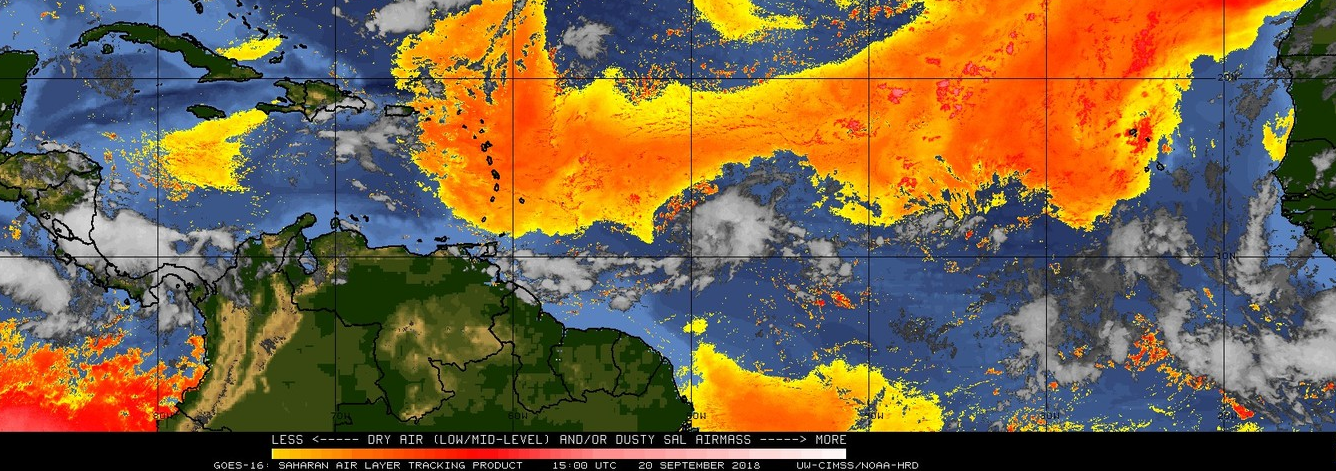
\includegraphics{images/20180920.15.NWAtlantic.SALgoes16split.png}
\caption{Figure \ref{fig:split}: GOES-16 Split Window Difference on September 20, 2019}
\label{fig:split}
\end{figure}

\section{Summary}\label{conclusions}

\begin{itemize}
  \tightlist
  \item
    The Saharan Air Layer (SAL) can be seen from space using visible and infrared imagery and products. Hyperspectral sounding data can be used to see both the vertical and horizontal extent in near real-time.
  \item
    NUCAPS is useful for examining the moisture and temperature structure of SAL events.
  \item
    Both code and web-based tools are useful for visualizating the SAL. For researchers, Suomi NPP and NOAA-20 NUCAPS are available via \href{https://www.bou.class.noaa.gov/saa/products/search?sub_id=0\&datatype_family=JPSS_SND\&submit.x=24\&submit.y=7}{NOAA
    CLASS} with a three-hour latency. For operational forecasters, NOAA-20 NUCAPS is available within 20 minutes in AWIPS.
  \end{itemize}
\end{document}
